\documentclass[../../main.tex]{subfiles}
\begin{document}

{\bf [解答]}
\paragraph{(1)}

% TODO: y=h(x)のグラフ．y=1,y=-1でグラフが綺麗に箱に入る様子を示す
\begin{figure}[htb]
  \centering
  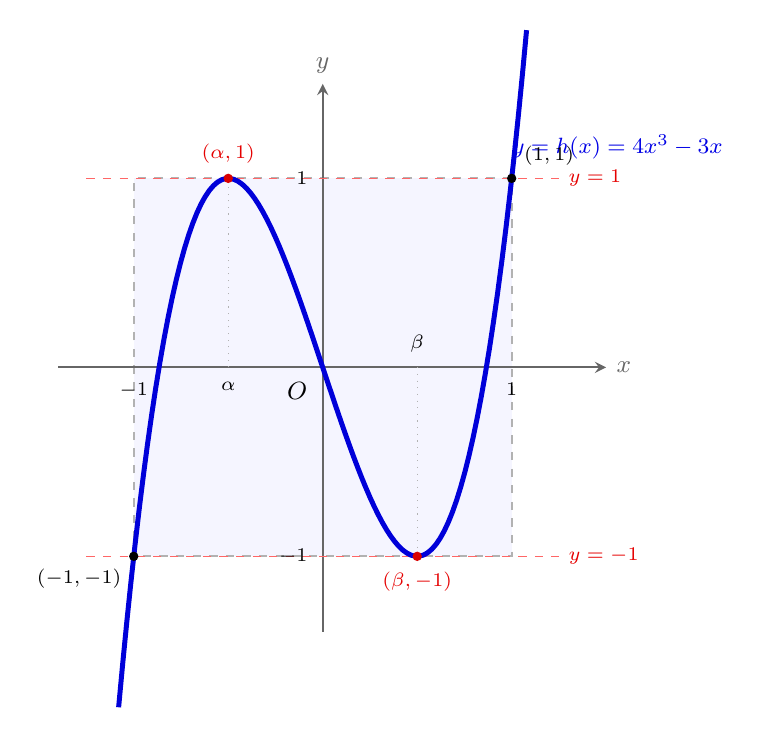
\begin{tikzpicture}[scale=2.4, >=stealth, every node/.style={font=\small}]

    % --- 1. 箱 [-1, 1] x [-1, 1] の背景と枠線 ---
    \fill[blue!5, opacity=0.8] (-1, -1) rectangle (1, 1);
    \draw[dashed, gray!60, thick] (-1, -1) rectangle (1, 1);

    % --- 2. 座標軸 ---
    \draw[->, thick, gray!80!black] (-1.4, 0) -- (1.5, 0) node[right] {$x$};
    \draw[->, thick, gray!80!black] (0, -1.4) -- (0, 1.5) node[above] {$y$};
    \node[below left=2pt] at (0, 0) {$O$};

    % --- 3. 水平・垂直の目盛り線 ---
    \draw[dashed, red!60] (-1.25, 1) -- (1.25, 1) node[right, font=\scriptsize, red!90!black] {$y = 1$};
    \draw[dashed, red!60] (-1.25, -1) -- (1.25, -1) node[right, font=\scriptsize, red!90!black] {$y = -1$};

    % --- 4. 曲線 y = h(x) = 4x^3 - 3x ---
    \draw[line width=1.8pt, blue!85!black, domain=-1.08:1.08, samples=100]
    plot (\x, {4*\x*\x*\x - 3*\x});
    \node[blue!90!black, font=\footnotesize\bfseries, above right] at (0.95, 1.05)
    {$y = h(x) = 4x^3 - 3x$};

    % --- 5. 接触点・極値点のプロットと投影破線 ---
    % 極大点 (-1/2, 1)
    \draw[dotted, gray!60] (-0.5, 0) -- (-0.5, 1);
    \node[circle, fill=red!85!black, inner sep=1.2pt] at (-0.5, 1) {};
    \node[above=2pt, font=\scriptsize, red!90!black] at (-0.5, 1) {$\left(\alpha, 1\right)$};
    \node[below=2pt, font=\scriptsize] at (-0.5, 0) {$\alpha$};

    % 極小点 (1/2, -1)
    \draw[dotted, gray!60] (0.5, 0) -- (0.5, -1);
    \node[circle, fill=red!85!black, inner sep=1.2pt] at (0.5, -1) {};
    \node[below=2pt, font=\scriptsize, red!90!black] at (0.5, -1) {$\left(\beta, -1\right)$};
    \node[above=2pt, font=\scriptsize] at (0.5, 0) {$\beta$};

    % 端点 (-1, -1), (1, 1)
    \node[circle, fill, inner sep=1.2pt] at (-1, -1) {}; \node[below left=1pt, font=\scriptsize] at (-1, -1) {$(-1, -1)$};
    \node[circle, fill, inner sep=1.2pt] at (1, 1) {}; \node[above right=1pt, font=\scriptsize] at (1, 1) {$(1, 1)$};

    % 軸目盛り
    \node[left=2pt, font=\scriptsize] at (0, 1) {$1$};
    \node[left=2pt, font=\scriptsize] at (0, -1) {$-1$};
    \node[below=2pt, font=\scriptsize] at (1, 0) {$1$};
    \node[below=2pt, font=\scriptsize] at (-1, 0) {$-1$};

  \end{tikzpicture}
  \caption{$y = h(x)$ のグラフの概形}
  \label{fig:chebyshev_box_hx}
\end{figure}

$-1 < x < 1$ で $h(x)$ が極大値を取る$x$を$\alpha$，極小値を取る$x$を$\beta$とおくと，題意より
\begin{align}
  \begin{cases}
    h(1)=h(\alpha)=1 \\
    h(-1)=h(\beta)= -1 \\
    h'(\alpha)=h'(\beta) = 0
  \end{cases}
\end{align}
である．よって因数定理より
\begin{align}
  \begin{cases}
    h(x) - 1 &= p(x-1)(x-\alpha)^2 \\
    h(x) + 1 &= p(x+1)(x-\beta)^2
  \end{cases} \label{eq:1}
\end{align}
と書ける．第一式を$x$で微分して
\begin{align}
  h'(x) = p(x-\alpha)^2 + 2p(x-1)(x-\alpha) = p(x-\alpha)(3x - \alpha - 2)
\end{align}
である．これが$h'(x)=p(x-\alpha)(x-\beta)$と等しいから，
\begin{align}
  \beta = \dfrac{\alpha+2}{3} \label{eq:2}
\end{align}
である．\cref{eq:1}の第二式にに代入して
\begin{align}
  h(x) + 1 = p(x+1)\Bigl(x - \dfrac{\alpha+2}{3}\Bigr)^2
\end{align}
だから，\cref{eq:1}の第一式と係数を比較して
\begin{align}
  \begin{cases}
    \text{2次}: p\Bigl(1 - \dfrac{2\alpha+4}{3}\Bigr) = p(-1-2\alpha) \\
    \text{定数}: 1 - \dfrac{1}{4}p = -1 + \dfrac{4}{9}p
  \end{cases}
\end{align}
である．$p\neq 0$に注意して整理すると
\begin{align}
  \begin{cases}
    \alpha = -\dfrac{1}{2} \\
    p = 4
  \end{cases} \label{eq:3}
\end{align}
である．これを\cref{eq:1}に代入して求める関数は
\begin{align}
  h(x) = 4(x-1)\Bigl(x + \dfrac{1}{2}\Bigr)^2 + 1 = 4x^3 - 3x \label{eq:4}
\end{align}
である．

\paragraph{(2)}

\begin{figure}[htb]
  \centering
  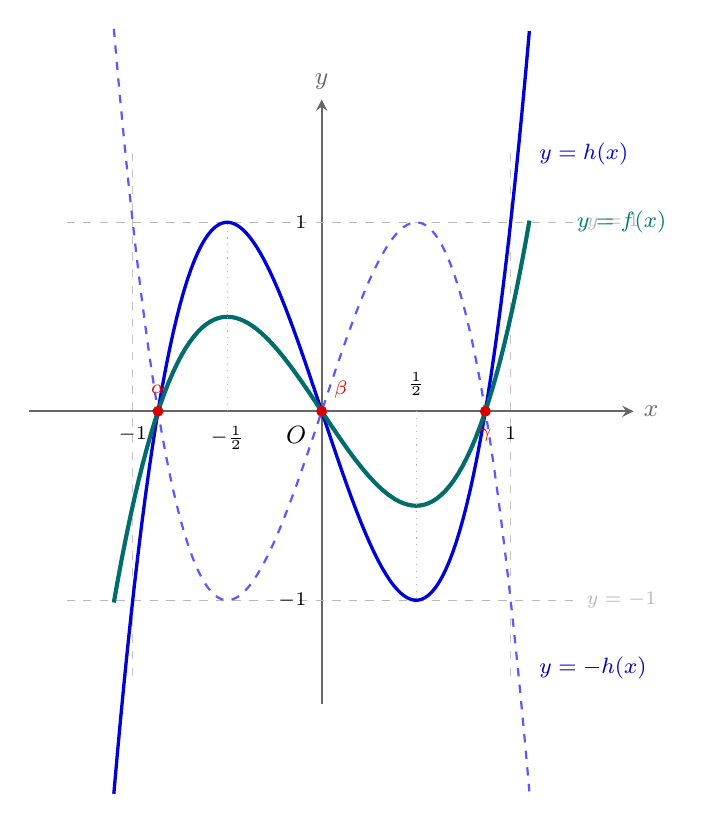
\begin{tikzpicture}[scale=2.4, >=stealth, every node/.style={font=\small}]

    % --- 1. 座標定義 (厳密な交点: y = 0 上) ---
    % alpha = -sqrt(3)/2 ≈ -0.8660
    % beta  = 0
    % gamma =  sqrt(3)/2 ≈  0.8660
    \pgfmathsetmacro{\sqThreeHalf}{sqrt(3.0)/2.0}

    \coordinate (O)        at (0, 0);
    \coordinate (Pt_alpha) at (-\sqThreeHalf, 0);
    \coordinate (Pt_beta)  at (0, 0);
    \coordinate (Pt_gamma) at (\sqThreeHalf, 0);

    % --- 2. 座標軸 ---
    \draw[->, thick, gray!80!black] (-1.55, 0) -- (1.65, 0) node[right] {$x$};
    \draw[->, thick, gray!80!black] (0, -1.55) -- (0, 1.65) node[above] {$y$};
    \node[below left=2pt] at (O) {$O$};

    % --- 3. 境界線 y = ±1, x = ±1 ---
    \draw[dashed, gray!55] (-1.35, 1) -- (1.35, 1) node[right, font=\scriptsize] {$y = 1$};
    \draw[dashed, gray!55] (-1.35, -1) -- (1.35, -1) node[right, font=\scriptsize] {$y = -1$};
    \draw[dashed, gray!45] (1, -1.4) -- (1, 1.4);
    \draw[dashed, gray!45] (-1, -1.4) -- (-1, 1.4);

    % --- 4. 曲線 y = h(x) と y = -h(x) ---
    % y = h(x) = 4x^3 - 3x (青実線)
    \draw[very thick, blue!85!black, domain=-1.1:1.1, samples=120]
    plot (\x, {4*\x*\x*\x - 3*\x});
    \node[blue!90!black, font=\footnotesize\bfseries, above right] at (1.1, 1.25) {$y = h(x)$};

    % y = -h(x) = -(4x^3 - 3x) (青破線)
    \draw[thick, dashed, blue!65, domain=-1.1:1.1, samples=120]
    plot (\x, {-(4*\x*\x*\x - 3*\x)});
    \node[blue!75!black, font=\footnotesize, below right] at (1.1, -1.25) {$y = -h(x)$};

    % --- 5. 条件を満たす具体的な 3 次関数 y = f(x) ---
    % f(x) = 2x^3 - 1.5x (緑太線)
    % ※ [-1, 1] で |f(x)| <= 1/sqrt(2) ≈ 0.707 < 1
    \draw[line width=1.5pt, teal!85!black, domain=-1.1:1.1, samples=100]
    plot (\x, {2.0*\x*\x*\x - 1.5*\x});
    \node[teal!95!black, font=\footnotesize\bfseries, right] at (1.3, 1.0)
    {$y = f(x)$};

    % --- 6. 厳密な 3 つの交点 alpha, beta, gamma のプロット ---
    \node[circle, fill=red!85!black, inner sep=1.4pt] at (Pt_alpha) {};
    \node[circle, fill=red!85!black, inner sep=1.4pt] at (Pt_beta) {};
    \node[circle, fill=red!85!black, inner sep=1.4pt] at (Pt_gamma) {};

    \node[above=3pt, font=\scriptsize\bfseries, red!90!black] at (Pt_alpha) {$\alpha$};
    \node[above right=1pt, font=\scriptsize\bfseries, red!90!black] at (Pt_beta) {$\beta$};
    \node[below=3pt, font=\scriptsize\bfseries, red!90!black] at (Pt_gamma) {$\gamma$};

    % --- 7. 目盛りと投影破線 ---
    % x = -1/2, 1/2 の極大・極小点
    \draw[dotted, gray!60] (-0.5, 0) -- (-0.5, 1);
    \draw[dotted, gray!60] (0.5, 0) -- (0.5, -1);
    \node[below=2pt, font=\scriptsize] at (-0.5, 0) {$-\frac{1}{2}$};
    \node[above=2pt, font=\scriptsize] at (0.5, 0) {$\frac{1}{2}$};

    % 境界目盛り
    \node[left=2pt, font=\scriptsize]  at (0, 1) {$1$};
    \node[left=2pt, font=\scriptsize]  at (0, -1) {$-1$};
    \node[below=2pt, font=\scriptsize] at (1, 0) {$1$};
    \node[below=2pt, font=\scriptsize] at (-1, 0) {$-1$};

  \end{tikzpicture}
  \caption{$y=h(x), -h(x)$ と任意の関数 $f(x)$ の交差および $|x|>1$ での大小関係}
  \label{fig:chebyshev_extremal_comparison_exact}
\end{figure}

$y=f(x), h(x)$ は連続な関数で，$-1 < f(x) < 1, -1 \le h(x) \le 1$を満たす．
また(1)から
\begin{align}
  \begin{cases}
    h(-1) = h(-1/2) = -1 \\
    h(1)  = h(1/2)  = 1
  \end{cases}
\end{align}
である．従って$y=f(x),h(x)$は$-1 < x < -\dfrac{1}{2}, \, -\dfrac{1}{2} < x < \dfrac{1}{2}, \, \dfrac{1}{2} < x < 1$ でそれぞれ交わる．
$f, h$ は3次関数だから，$g(x) = f(x) - h(x)$ と定めるとこれも高々$3$次関数である．そこで適当な $0$ でない定数 $k$ と，
\begin{align}
  -1 < \alpha < -\dfrac{1}{2} < \beta < \dfrac{1}{2} < \gamma < 1 \label{eq:5}
\end{align}
をみたす $\alpha, \beta, \gamma$ において
\begin{align}
  g(x) = f(x) - h(x) = k(x-\alpha)(x-\beta)(x-\gamma) \label{eq:6}
\end{align}
とおける．

まず$k$の符号について，$x=1/2$とすると
\begin{align}
  \begin{cases}
    g(1/2) = f(1/2) +1 > 0 \\
    (1/2-\alpha)(1/2-\beta)(1/2-\gamma) < 0
  \end{cases}
\end{align}
より，$k<0$である．

したがって$g(x)$の符号について
\begin{align}
  \begin{cases}
    1 < x  \text{ においては}，g(x) < 0 \\
    x < -1 \text{ においては}，g(x) > 0
  \end{cases}
  \iff
  \begin{cases}
    1 < x \text{ の時}，h(x) > f(x) \\
    x < -1 \text{ の時}，h(x) < f(x)
  \end{cases} \label{eq:7}
\end{align}
である．

$P(x) = f(x) + h(x)$ についても同様の議論から，
\begin{align}
  \begin{cases}
    1 < x \text{ の時}，-h(x) < f(x) \\
    x < -1 \text{ の時}，f(x) < -h(x)
  \end{cases} \label{eq:8}
\end{align}
である．

\cref{eq:7,eq:8}から
\begin{align}
  |x| > 1 \text{ の時 } |f(x)| < |h(x)|
\end{align}
である．

% TODO
% % --- 6. 注釈ボックス ---
%   \node[draw=blue!85!black, fill=white, rounded corners=2pt, inner sep=3.5pt, font=\footnotesize, align=left]
%     at (0, -1.65) {
%       \textbf{第 $1$ 種チェビシェフ多項式 $h(x) = T_3(x)$ の性質}:\\[2pt]
%       $\bullet\ -1 \le x \le 1$ において $-1 \le h(x) \le 1$（箱の中に完全に収まる）\\[2pt]
%       $\bullet\ 4$ 箇所で境界 $\pm 1$ に等振幅で接触（交替定理の極値点）
%     };

\end{document}
